\documentclass[letterpaper,twoside,12pt]{article}
\usepackage[dvips]{graphicx}
\usepackage[margin=0.8in]{geometry}
\usepackage{caption}
\usepackage{amsmath}
\usepackage{amssymb}
\usepackage[T1]{fontenc}
\usepackage{natbib}
\usepackage{authblk}
%\usepackage{fancyvrb}
%\usepackage{lmodern}
%\usepackage{url}
%\usepackage{times}
\usepackage{textcomp}
%\usepackage{parskip}
\bibliographystyle{agu08}

\newcommand{\ud}{\mathrm d}
\newcommand{\uj}{\mathrm{j}}
\newcommand{\bz}{\mathbf{z}}
\newcommand{\Real}{\mathrm{Re}}
\newcommand{\Imag}{\mathrm{Im}}
\newcommand{\dif}{\mathrm{d}}
\newcommand{\sigsig}{\sigma_1\sigma_2}
\newcommand{\varss}{\varsigma_1\varsigma_2}
\newcommand{\hvarss}{\hat{\varsigma}_1 \hat{\varsigma}_2}
\newcommand{\twodots}{\mathinner {\ldotp \ldotp}}
\newcommand{\midtilde}{\raisebox{0.5ex}{\texttildelow}}

\DeclareMathOperator\erf{erf}

\title{Normality Test for 2-bit Stream Data in Mark-5 Files}

\author[1]{L. V. Benkevitch}
\affil[1]{\small MIT Haystack observatory, Westford, MA 01886, USA.}


\begin{document}

\maketitle

\begin{abstract}
The radio astronomy data from a single dish are recorded in M5B (Mark-5) or VDIF formatted files. The recorded data are supposed to be Gaussian white noise. A corrupted data segment can be spotted at the output of correlation stage. However, the correlation is expensive and vastly increases the bulk of data to be analyzed for spurious parts. Here we consider a problem of finding non~Gaussian (or non-normal) single-dish data segments in M5B files.

The problem may be thought about from a security standpoint. Suppose someone (a malicious character) wishes to hack a system and figures an approach would be to embed some malicious code in. Is it possible to detect the embedded (non-Gaussian) data within a frame or multiple frames before the correlator? Also, even though an algorithm can be determined, is it possible to make its implementation fast enough? The data files are large (up to a hundred gigabytes).

Our solution is based on Pearson's $\chi^2$ test. The null hypothesis states that the data in file  are consistent with the normal distribution. If the data in a part of the file do not pass the test at the significance level 0.05, the null hypothesis is rejected, and the data fragment is flagged.

The algorithm runs on the GPU (Graphics Processing Unit), which provides high speed computations.
\end{abstract}


\tableofcontents

\section{Signal Quantization and M5B Data Structure}

The analog signal from a single antenna/dish is supposed to be Gaussian noise with the expectation $\mu$ and standard deviation (rms) $\sigma$ distributed according to the normal law with the probability density function (PDF):

\begin{equation}
  \label{normal_pdf}
  N(\mu,\sigma) =  \frac{1}{\sigma\sqrt{2\pi}} e^{-\frac{(x-\mu)^2}{2\sigma^2}}.
\end{equation}

The signal is centered to ensure zero $\mu$ and its band is filtered into 16 frequency channels each of which is passed through the 4-level quantizer with the characteristic shown in Fig.~\ref{quant4lvl}.  The quantizer has just three switching thresholds, $-\theta$, 0, and $\theta$, so it is characterized with the only parameter, the adjustable quantization threshold $\pm\theta$. Note that the hardware deals with voltage thresholds, $\pm v_0$, but $\theta$ is expressed in the signal STDs, thus it is dimensionless, $\theta = v_0/\sigma$. The quantizer output only takes four values as in Tab.~\ref{quant_io}. These values are saved in the M5B file.


\begin{figure}[ht!]
  \begin{center}
  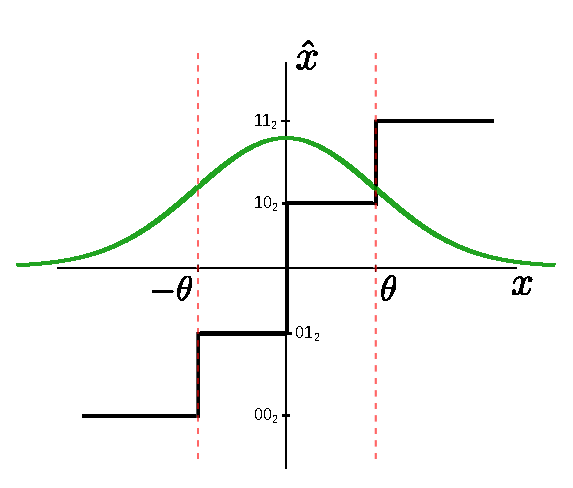
\includegraphics[width=25pc]{fig_4_Level_Quantization_Pattern_impr.eps}
  %\noindent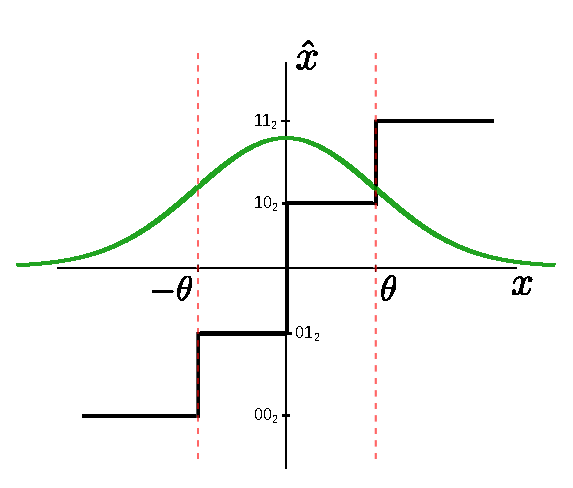
\includegraphics[width=20pc]{fig_4_Level_Quantization_Pattern_impr.eps}
  %\includegraphics[width=\linewidth]{}
  \caption{\small The 4-level quantizer characteristic is shown as a black polygonal line. The input analog signal $x$, distributed normally, can take any value in $(-\infty \twodots +\infty)$. In response to $x$, the quantizer outputs $\hat{x}$ with only four values, 0, 1, 2, and 3, according to Tab.~\ref{quant_io}. The normal probability density function (PDF) of $x$ is shown as a green line.}
  \label{quant4lvl}
  \end{center}
\end{figure}


\begin{table}[ht!]
  \begin{center}
    \caption{Quantizer Characteristic}
    \label{quant_io}
    \begin{tabular}{c|c}
      \textbf{Input, $x$} & \textbf{Output, $\hat{x}$} \\
      \hline
      $-\infty$ to $-\theta$ & 0 \\
      $-\theta$ to 0         & 1 \\
      0 to $\theta$          & 2 \\
      $\theta$ to $+\infty$  & 3 \\
    \end{tabular}
  \end{center}
\end{table}


The M5B file can be considered as an array of 10016-byte frames. Each frame consists of 2504 32-bit words (\verb@unsigned int@ or  \verb@uint@ in C/C++). The first 4 words comprise the frame header, so a frame has 2500 words of pure data. Each 32-bit data word is subdivided into 16 2-bit channels, numbered from 0 to 15. The header contains the sync word \verb@0xABADDEED@, 23-bit long frame number within second (reset to zero each new second), one flag bit to tag the frame invalid, 8-bit long channel ID, BCD Time Code Word 1 (‘JJJSSSSS’), BCD Time Code Word 2 (‘.SSSS’), and  16-bit CRCC.

Unfortunately, the frame headers do \emph{not} contain the quantization threshold values $\theta = v_0/\sigma$ necessary for the statistical testing. In order to estimate $\theta$, the algorithm has to spend precious time on its 1D search as will be described further. 




\section{Statistical Testing Data Normality Using $\chi^2$}

We need to test if the data in each of the 16 channels are sampled from a normally distributed population (the null hypothesis) or not (the alternative hypothesis). In each frame and channel, there are $N=$ 2500 data samples divided into $n=4$ categories by their values, 0, 1, 2, and 3. The counts of data samples in each category form the 4 histogram bins $B_i, i=\overline{0 \twodots 3}$, so $\sum_{i=0}^3 B_i = N$. The Pearson's $\chi^2$ test is based on comparing the observed data counts with the expected (theoretical) counts $E_i, i=\overline{0 \twodots 3}$ obtained from the normal PDF~\eqref{normal_pdf} as $E_i = Np_i$. Here $p_i$ is the probability that a random value sampled from $N(0,\sigma)$ is within the $i$-th interval. The intervals are given in Tab.~\ref{quant_io}, where $i$ is one of the Output values. $\ldots\cdots\ldotp\ldotp$

For each data frame the value of the test-statistic is calculated as

\begin{equation}
  \label{x2_calc}
  X^2 = \sum_{i=0}^3 \frac{(B_i - E_i)^2}{E_i}.
\end{equation}


The $X^2$ test statistic asymptotically approaches the $\chi^2_{k=3}$ distribution, where $k = n - 1 = 3$ is the number of degrees of freedom. The $\chi^2_{k=3}$ PDF is shown in Fig.~\ref{chi2_pdf}. The statistic $X^2$ is a random value showing how close are the observation frequencies $B_i$ to the perfect, theoretical frequencies $E_i$. The $\chi^2_{k=3}$ PDF has maximum at $X^2=1$ and the mean at $X^2=k=3$. This means that if $X^2$ is distributed as $\chi^2_{k=3}$ its most probable random values will be concentrated somewhere around the mean 3 and not much further. But how much further? The area under the $\chi^2_{k=3}$ PDF curve in Fig.~\ref{chi2_pdf} over an interval $[a,b]$ equals to the probability that the random value will appear within this interval. If we want to be 95\% confident that the data is distributed normally, $X^2$ cannot exceed the critical value $\chi^2_{cr}$ such that the probability for $X^2$ to appear within the interval $[0 \twodots \chi^2_{cr}]$ is $p=0.95$. The critical $\chi^2_{k=3}$ value can be calculated as the value of $\chi^2$ Probability Point Function or PPF, the inverse of the $\chi^2$ Cumulative Distribution Function or CDF. In Python this is done as $\verb@scipy.stats.chi2.ppf(1-alpha, k)@$, where $\alpha = 0.05$ is the level of significance. In our case $\chi^2_{cr} = 7.81$. 

\begin{figure}[ht!]
  \begin{center}
  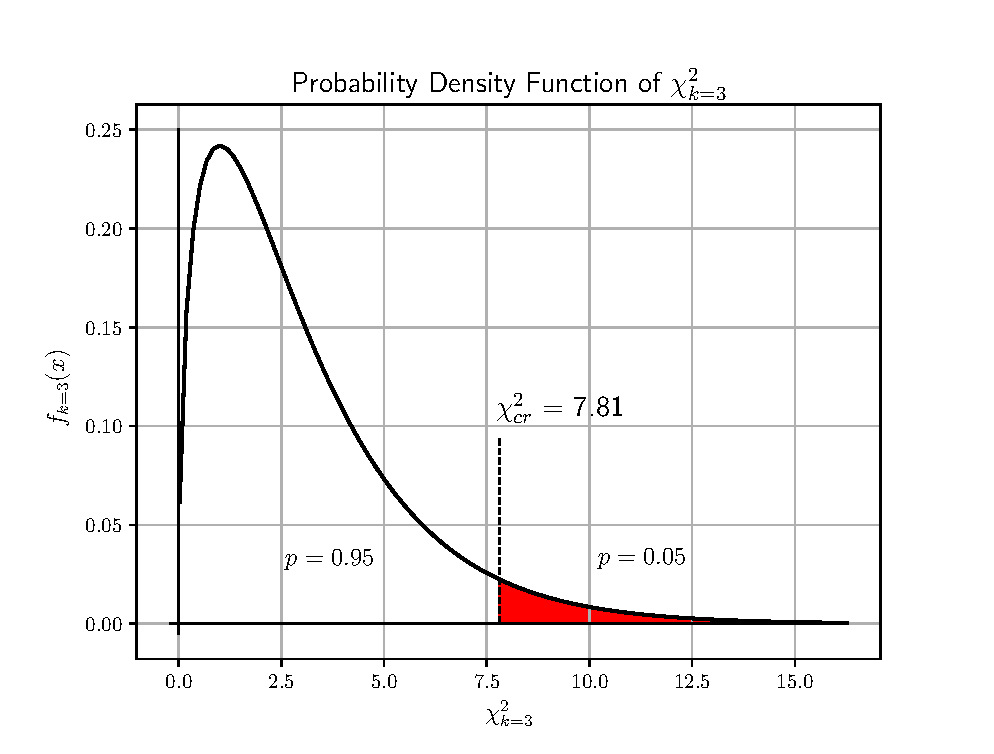
\includegraphics[width=30pc]{fig_chi2_pdf.eps}
  %\noindent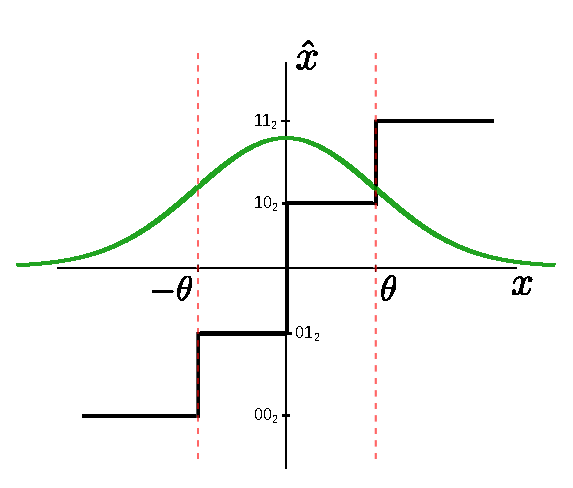
\includegraphics[width=20pc]{fig_4_Level_Quantization_Pattern_impr.eps}
  %\includegraphics[width=\linewidth]{}
  \caption{\small Chi-squared probability density function (PDF). The red area under the curve to the left of $\chi^2_{cr} = 7.81$ equals the probability $p=0.05$. This is the probability that the $X^2$ statistic (Eq.~\eqref{x2_calc}) for normal $B_i$ exceeds 7.81.}
  \label{chi2_pdf}
  \end{center}
\end{figure}

Thus, our algorithm flags a channel data in frame as non-Gaussian if its $X^2 > 7.81$, the probability of incorrectly rejecting the null hypothesis being $\alpha = 0.05$. In Fig.~\ref{chi2_pdf} this is the red-filled area with the probability 0.05 over the range $[\chi^2_{cr} \twodots +\infty)$. 



\section{Estimation of Quantization Threshold Using 1D Search}

As mentioned, the M5B files do not provide the values of quantization threshold $\theta$, which is continuously being adjusted and can differ from one frame to the next. Assuming the data are sampled from the normally distributed population we can hypothesize that the $\theta_{\text{opt}}$ value that provides the best fit of the observed frequencies $B_i$ to the normal frequencies $E_i$ can be a good estimate of the actual $\theta$ established at the quantization time.

One can notice that the $X^2$ statistics in Eq.~\eqref{x2_calc} is a function of a single variable $\theta$: 

\begin{equation}
  \label{x2_func_of_theta}
  X^2(\theta) = \sum_{i=0}^3 \frac{(B_i - E_i(\theta))^2}{E_i(\theta)},
\end{equation}

\noindent where the normal frequencies $E_i$ are dependent on the positions of quantization thresholds:

\begin{equation*}
  \label{norm_freq}
  E_{0\twodots3}(\theta) = N \cdot \left[\Phi(-\theta); \; \; \; \frac{1}{2}-\Phi(-\theta);  \;\;\; 
                             \frac{1}{2}-\Phi(-\theta); \; \; \; \Phi(-\theta) \right],
\end{equation*}

\noindent as shown in Fig.~\ref{npdf_areas}, and $\Phi(x)$ is the normal CDF with $\mu=0$ and $\sigma=1$:

\begin{equation}
  \label{ncdf}
  \Phi(x) = \frac{1}{2} \left[1 + \erf \left( \frac{x}{\sqrt{2}} \right) \right].
\end{equation}


\begin{figure}[ht!]
  \begin{center}
  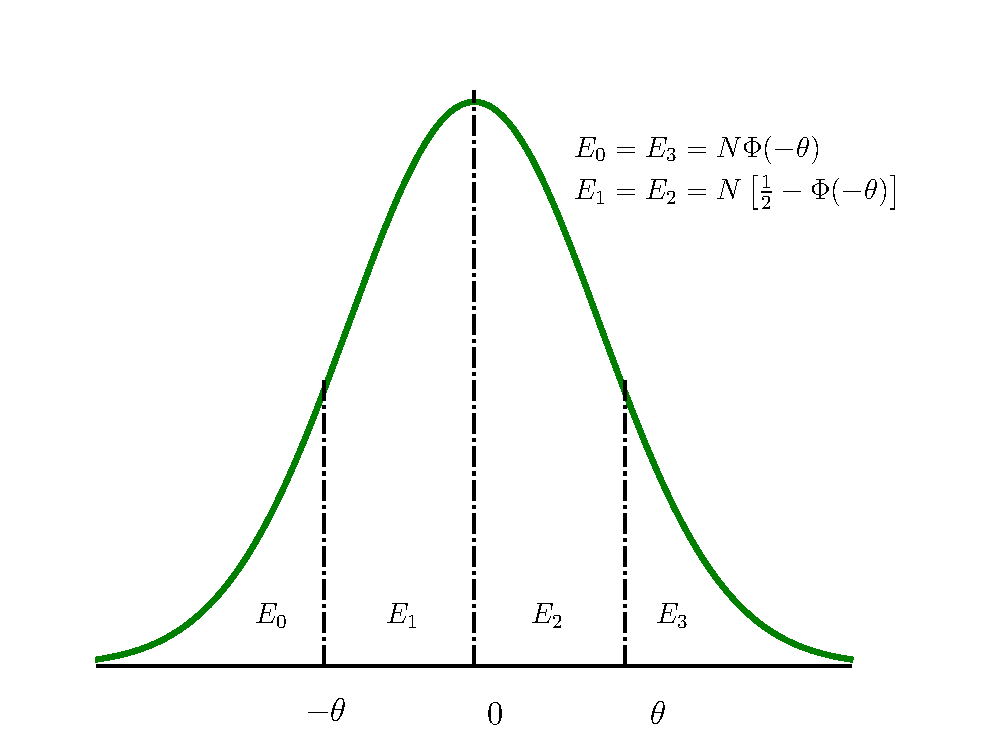
\includegraphics[width=30pc]{fig_npdf_areas.eps}
  \caption{\small The normal frequencies $E_i$ are dependent on the quantization thresholds $\pm\theta$. They are calculated with the use of normal cumulative distribution function (CDF) given in Eq.~\eqref{ncdf}.}
  \label{npdf_areas}
  \end{center}
\end{figure}

Fig.~\ref{optimum_theta} shows that the curve $y = X^2(\theta)$ has the only minimum. Thus, the best fit of the normal frequencies $E_i$ to the observed frequencies $B_i$ can be reached at the single $\theta=\theta_\text{opt}$ value that provides minimum to $X^2(\theta)$. 

We have used a fast-converging Brent's algorithm for one-dimensional search. It is a combination of the golden section search at the beginning and the parabolic interpolation when the process is close enough to the minimum.


\begin{figure}[ht!]
  \begin{center}
  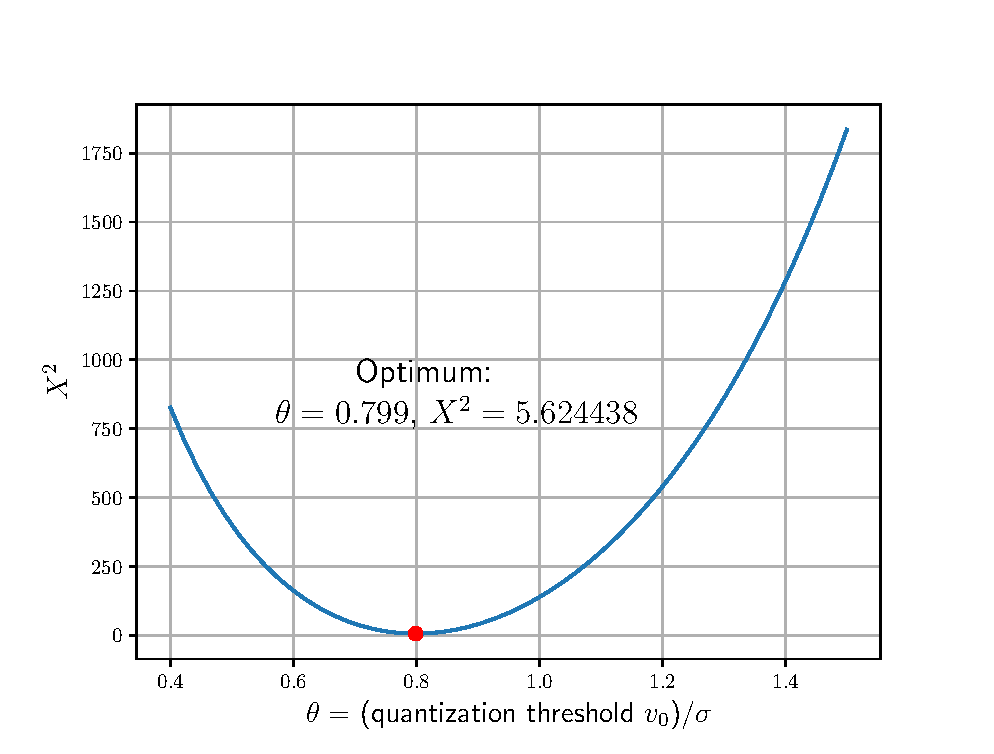
\includegraphics[width=30pc]{fig_optimal_quantization_threshold.eps}
  \caption{\small $X^2(\theta)$ from Eq.~\eqref{x2_func_of_theta} as the measure of error between the observed, $B_i$, and normal, $E_i$ frequencies for the range of quantization tresholds $[0.4 \mathinner{\ldotp\ldotp}1.5]$. The curve has minimum at $\theta = 0.7988$, which can be used as an estimate for the actual threshold used in the analog signal quantization.}
  \label{optimum_theta}
  \end{center}
\end{figure}


\section{Using Graphics Processing Units (GPU)}

The Graphics Processing Units with their hundreds and thousands of processor cores and multiple memory channels allow 1 to 3 orders of magnitude speed-up of the common algorithms. There are two major software frameworks, CUDA and OpenCL. CUDA is developed specifically for the Nvidia GPUs. OpenCL can be used on many parallel architectures. OpenCL is the only option for the AMD GPUs.

In both frameworks, the application code consists of two parts. One part is executed on the host PC. It reads the M5B files, prepares the GPU, uploads there the codes and the M5B data, starts the computations on the GPU, downloads the results from the GPU to the host memory, and saves them to the disk. The other part of code is executed in parallel on the multiple GPU cores. The programs executed on the GPU are called kernels. 

In both frameworks we use single precision floating point arithmetics, which provides the fastest computations.

In the both frameworks, the kernels are written in the C language subsets with some extensions. The host code uses CUDA or OpenCL API. It can be written in C/C++ and some other languages. However, Python is always preferred to make life easier. We use Python wrappers for the both frameworks: PyCUDA and PyOpenCL, and the host part of the NormTest software is written in Python. 

The Python module for normality testing, \verb@gpu_m5b.py@, described in the next section, transfers control to the C kernel previously transferred to the GPU. The kernels are different for different frameworks used. In any individual normality test only two C files are used. Their names start with the strings \verb@"ker_m5b_gauss_test"@ and \verb@"fminbndf"@: \\

\noindent \verb@ker_m5b_gauss_test*@ defines the test kernel \verb@m5b_gauss_test()@ and the minimized function  \\
\hangindent=0.7cm \verb@calc_chi2()@, which calculates $\chi^2$ between the four bins of standard normal distribution and the four bins with the observation data counts. \\

\noindent \verb@fminbndf*@ implements one-dimensional search for the optimal quantization threshold $\theta_\text{opt}$  \\
\hangindent=0.7cm based on Brent's algorithm. It calls the \verb@calc_chi2()@ function. The search is performed within the bounds $\theta \in [0.5\sigma \twodots 1.5\sigma]$ with the absolute precision \verb@atol@ $=10^{-4}$. Also, the number of iterations is limited to  \verb@maxiter = 20@. \\


In the CUDA framework just the two C files are used: \\

\noindent \verb@ker_m5b_gauss_test.cu@  - test kernel for CUDA; \\
\noindent \verb@fminbndf.cu@ - Brent's algorithm for CUDA. \\

The OpenCL framework requires more options because of the different implementations of OpenCL for different hardware platforms, AMD and Nvidia. Unfortunately, according to OpenCL Specifications, pointers to functions are not allowed, while CUDA does not have this restriction. So, in the OpenCL code for AMD GPU, instead of using this convenient mechanism to pass to the \verb@fminbndf()@ optimizer the pointer to an arbitrary minimized function as its parameter, we have to call \verb@calc_chi2()@ from inside \verb@fminbndf()@. This makes \verb@fminbndf()@ less universal. On the contrary, Nvidia's OpenCL implementation (probably) has an extension allowing this feature. Therefore, there are four OpenCL C files: \\

\noindent \verb@ker_m5b_gauss_test.cl@ - test kernel for Nvidia OpenCL; \\
\noindent \verb@fminbndf.cl@ - Brent's algorithm for Nvidia OpenCL, \\

\noindent and \\

\noindent \verb@ker_m5b_gauss_test_amd.cl@ - test kernel for AMD OpenCL; \\
\noindent \verb@fminbndf_amd.cl@ - Brent's algorithm for AMD OpenCL. \\

The parallel processing in kernels is organized framewise. As many frames as possible are uploaded and stored un the GPU RAM, and each one data frame is processed in one CUDA thread or in one OpenCL work item in parallel. The frames are independent of one another, so no thread synchronization is required. Within one thread/work item, though, the frame and its 16 channels are processed sequentially. The kernel finds the counts of channel data in each of the four bins, runs the 1D Brent's search for the optimal quantization threshold, calculates $\chi^2$ against the standard normal distribution, and saves the results in the output arrays. This is repeated until all the file chunks are processed.





\section{Python Module for Normality Testing gpu\_m5b.py}

The \verb@gpu_m5b.py@ module defines the only class \verb@Normtest@ that integrates in itself all the normality testing mechanisms. When imported from the \verb@gpu_m5b@ module, \verb@Normtest@ class probes the hardware and automatically determines which framework to use. If it detects an AMD GPU, it uses OpenCL. If an Nvidia GPU is detected, the software uses CUDA. In case both frameworks are installed, it prefers CUDA since it is \midtilde 1.5  times faster than OpenCL. Thus this class provides "transparent" access to the GPU independent of the software framework used. Current version of the software can use only one GPU, however, in future it is possible to employ multiple GPUs on the same motherboard, even using different frameworks. 

The \verb@Normtest@ class provides a "class method" \verb@do_m5b()@ with one mandatory, positional argument, a string with M5B filename, and an optional keyword argument, \verb@nthreads@: \\

\noindent \verb@Normtest.do_m5b(<M5B file name> [, nthreads=<# of threads in a block>])@ \\

 It runs the normality test on the available GPU using the software framework selected. If the M5B file is large and it does not fit into either the system RAM or the GPU RAM, it is processed in chunks. The \verb@Normtest@ class is not intended to create multiple class instances (although it is surely possible). Instead, the method \verb@do_m5b()@ is called directly with the class name or its alias. Below is an example procedure of normality tests on several M5B or M5A files: \\

\noindent
\verb@from gpu_m5b import Normtest as nt@  \\
\verb@nt.do_m5b("rd1910_wz_268-1811.m5b")@ \\
\verb@nt.do_m5b("rd1910_ny_269-1413.m5a")@ \\
\verb@nt.do_m5b("rd1910_ny_269-1404.m5a")@ \\
\verb@nt.do_m5b("rd1903_ft_100-0950.m5b")@ \\

The results are saved in 5 binary files. The files have the following names: \\\\
\verb@nt_<data>_<framework>_<m5b_basename>_<timestamp>.bin@, \\\\
\noindent where

\noindent \verb@<data>@ is one of the result types: \\
\indent \verb@hist:   dtype=np.float32, shape=(n_frames,16,4)@, 4 histogram bins for 16 channels; \\
\indent \verb@chi2:   dtype=np.float32, shape=(n_frames,16)@, $\chi^2$ for 16 channels; \\
\indent \verb@thresh: dtype=np.float32, shape=(n_frames,16)@, quantization thresholds found
        for 16 channels; \\
\indent \verb@flag:   dtype=np.uint16, shape=(n_frames,16)@, flags for 16 channels; \\
\indent \verb@niter:  dtype=np.uint16, shape=(n_frames,16)@, number of iterations of Brent's
        optimization method used to find the optimal quantization threshold
        for 16 channels;

\noindent \verb@<framework>@ is \verb@cuda@ or \verb@opencl@. \\
\noindent \verb@<m5b_basename>@ is the M5B or M5A file name without extension; \\
\noindent \verb@<timestamp>@ is \verb@YYYYMMDD_HHMMSS@ followed by milliseconds, like \verb@20231015_113649.078@. The timestamp is intended to make the result filename reasonably unique. \\

Empirically, it has been found that the best performance is achieved 
with 8 threads per block (in CUDA terminology), or, which is the same, 
8 work items per work group (in OpenCL terms). However, this number can 
be changed using the \verb@nthreads@ parameter. An example of setting 64 threads per block: \\

\noindent \verb@nt.do_m5b("rd1910_wz_268-1811.m5b", nthreads=64)@ 


\section{Data Flagging}

The binary files \verb@nt_flag*.bin@ created by \verb@Normtest.do_m5b()@ method contain flags for every channel in every frame. They are actually arrays of C/C++ \verb@unsigned short int@ or Python \verb@dtype=np.uint16@ with the dimensions \verb@[n_frames,16]@. The flags values mean the following conditions:
 
\indent 0: no errors; \\
\indent 1: bad frame signature; flags for all the channels are filled with 1.  \\
\indent 2: 1D search for the optimal quantization threshold did not converge in 20 iterations; \\
\indent 3: $\chi^2 > \chi^2_{cr}$.

\noindent Thus the flag value 3 can indicate that the frame contains some extraneous data other than the Gaussian data streams from a dish. The flags can be easily read in IPython into an array. For example: \\

\noindent \verb@fl = np.fromfile("nt_flag_cuda_rd1910_wz_268-1811_text_20231024_174438.173.bin", \@ \par
\noindent \verb@                 dtype=np.uint16)  # Read the flag file into 1D array fl;@ \par
\noindent \verb@fl = fl.reshape((len(fl)//16,16)) # Convert it into 2D array fl[n_frames,16]@  \par



\section{Python Scripts for Analysis of Results}

\subsection{inspect\_nt.py}

This script creates 4x4 plots of 16 histograms for each of the 16 channels. The plots are for one or several (averaged) frames. The histograms are compared with the normal distribution curves showing the vertical borders of the bins at the positions of quantisation threshold estimates, $\pm\theta$. In each subplot both $\theta$ and $\chi^2$ values are printed. The $\chi^2$ values exceeding $\chi^2_{cr} = 7.81$ are printed in red. The data are read from the \verb@*.bin@ files created with the \verb@gpu_m5b_chi2.py@. \\

\noindent Running: \\

\noindent \verb@%run inspect_nt.py <m5b_filename> <timestamp> <start_frame_#> <#_of_frames> @ \\

The \verb@<timestamp>@ can be any rightmost part of the timestamp before the file extension, \verb@.bin@. The timestamp is present in order to distinguish the \verb@*.bin@ files generated for the same M5B file at different runs. In most cases, providing the last 3 digis (i.e. milliseconds) is enough as long as they refer to the unique group of binary files with normality test results. \\

The histograms in Fig.~\ref{hists_good_4x4} are close to the normal histograms with good $\chi^2$ values, i.e. < 7.81. They are generated by \\

\noindent \verb@%run inspect_nt.py rd1910_wz_268-1811.m5b 575 1000 1@. \\

\begin{figure}[ht!]
  \begin{center}
  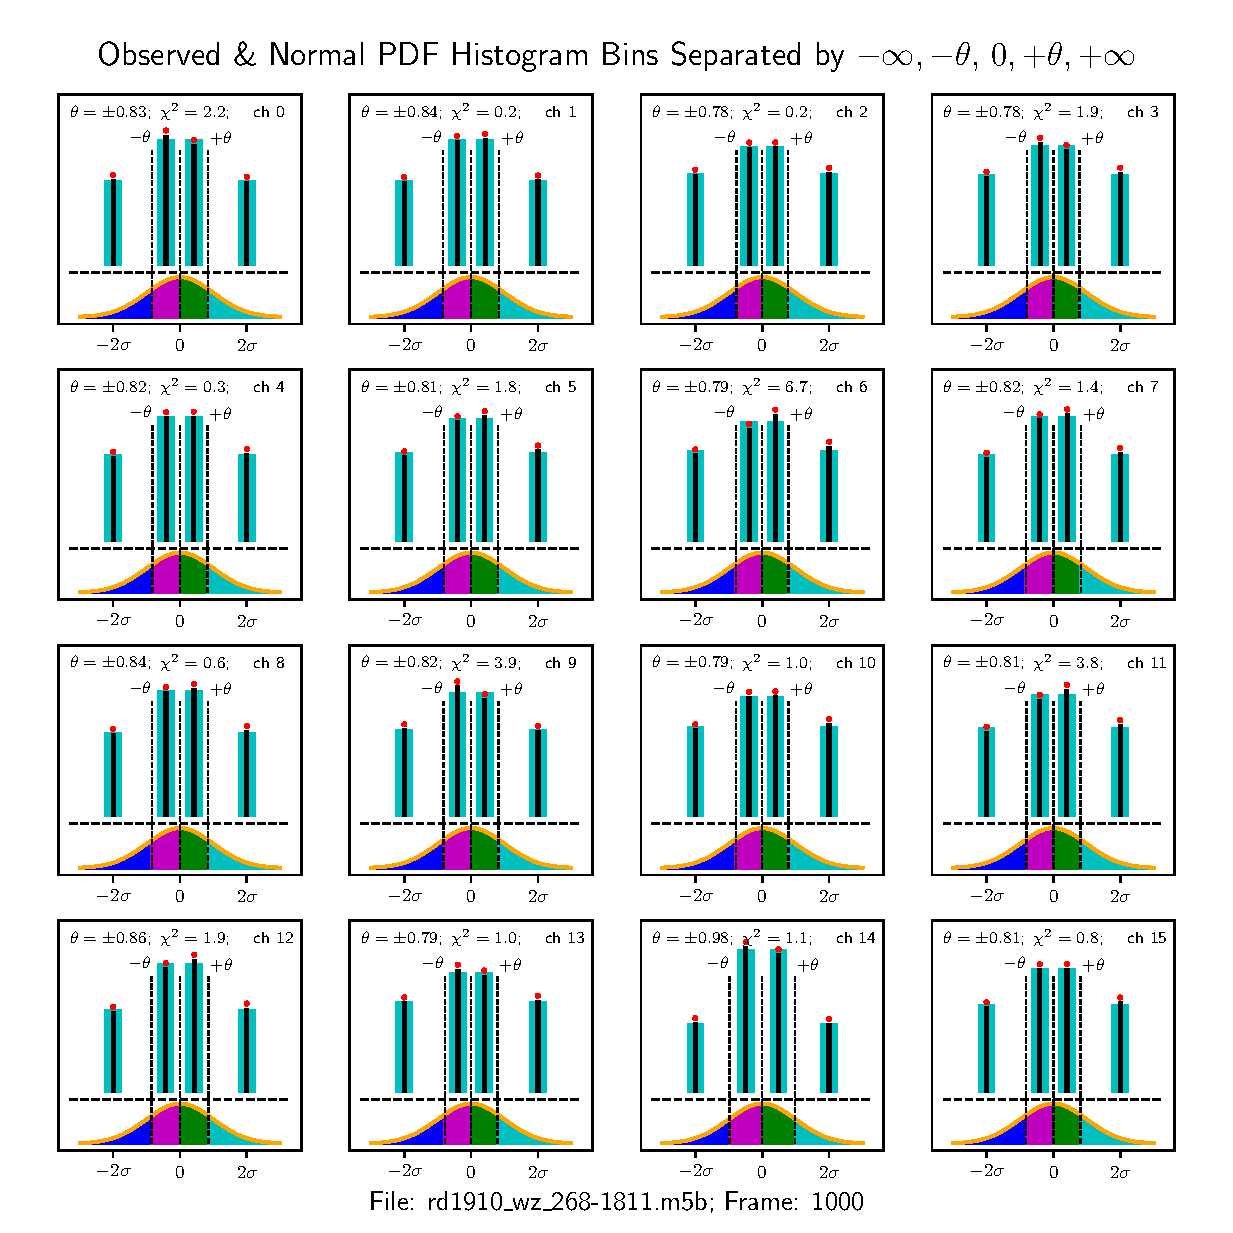
\includegraphics[width=40pc]{fig_4x4_Histograms_good.eps}
  %\noindent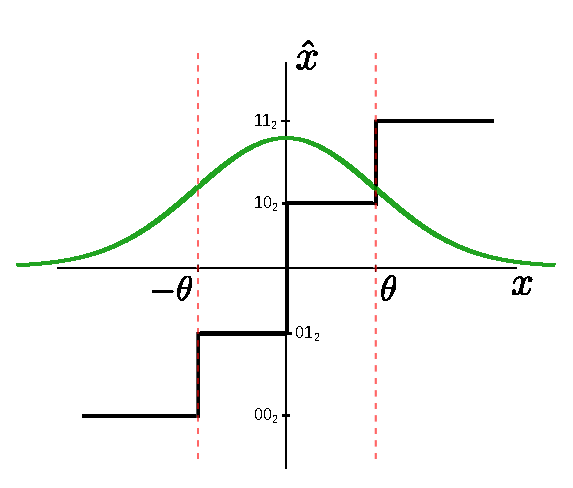
\includegraphics[width=20pc]{fig_4_Level_Quantization_Pattern_impr.eps}
  %\includegraphics[width=\linewidth]{}
  \caption{\small Observed and normal PDF histogram bins separated by $-\infty, -\theta, \, 0, +\theta, +\infty$. The histograms of observed data from an M5B file frame 1000 are shown as narrow black bars with red dots at the tips. The histograms of normal PDF are wider cyan bars. The normal PDFs with colored areas are given below the histograms. Here the observed distributions are close to the normal.}
  \label{hists_good_4x4}
  \end{center}
\end{figure}



\subsection{plot\_m5b\_hist.py}

Plots two histograms of the results from \verb@gpu_m5b.py@ for a whole M5B (or M5A) file.  Running: \\

\noindent \verb@%run plot_m5b_hist.py <M5B file name> <timestamp> @ \\

One histogram is the distribution of $\chi^2$ and a red marker showing position of the critical $\chi^2$ value,  $\chi^2_{cr} = 7.81$ at significance level 0.05, as well as the percent of $\chi^2$ exceeding it. The other is the distribution of the optimal quantization thresholds and a red marker showing position of the critical threshold value $\theta_{cr} = \pm 0.6745$ rms, as well as the percent of the thresholds that failed to reach it. The critical quantization threshold $\theta_{cr}$ is the one that separates 4 bins with equal areas under the normal curve. For $\theta = \theta_{cr}$ the histogram reflects the uniform distribution. 

Fig.~\ref{chi2_and_thresh_distr_1} and Fig.~\ref{chi2_and_thresh_distr_2} in Addendum show example plots generated by \\
\noindent \verb@%run plot_m5b_hist.py rd1903_ft_100-0950.m5b 025@ \\
\indent and \\
\noindent \verb@%run plot_m5b_hist.py rd1910_wz_268-1811.m5b 793@.


\subsection{Spotting Bad Frames with print\_frame\_chan\_chi2.py}

Sometimes a few channels in good data are flagged just because of random fluctuations in the data itself, and not because an alien piece of code was injected. Normally, in cases of fluctuations, $\chi^2$ only slightly exceeds its critical value $\chi^2_{cr} = 7.81$. In contrast, a really foreign piece of code or data damages the whole frame or many frames in a row, and the $\chi^2$ values in such bad frames are many times larger than $\chi^2_{cr}$. In order to spot such frames we should roughen the Pearson's $\chi^2$ criterion by searching for the frames where, say, $\chi^2 > 20$ or even 50. It can be done with the script \\

\noindent \verb@print_frame_chan_chi2.py <chi2 file name .bin> <chi2_threshold value>@ \\

\noindent For example:
\begin{verbatim}
%run print_frame_chan_chi2.py \
          nt_chi2_cuda_rd1910_wz_268-1811_bin_code_20231024_125630.067.bin 50.
\end{verbatim}

It is also easy to do by hand in \verb@IPython@. For example: 
\begin{verbatim}
import numpy as np
c2 = np.fromfile("nt_chi2_cuda_rd1910_wz_268-1811_text_20231024_174438.173.bin"
                 dtype=np.float32) # Read chi^2 into 1D array c2
c2 = c2.reshape((len(c2)//16,16)) # Convert it into 2D table c2[frame,chan]
ic = np.where(c2 > 50) # Find indices into c2 where chi^2 > 50
# Print a table of frame #, channel #, and chi^2 > 50:
for i in range(len(ic[0])):
    print(ic[0][i], ic[1][i], c2[ic[0][i],ic[1][i]])
\end{verbatim}

This will print something like
\begin{verbatim}
10 0 285.7461
10 1 314.56174
10 2 1594.8091
10 3 2500.0012
10 4 266.89368
10 5 338.24966
10 6 1693.4324
10 7 2500.0012
10 8 337.42603
10 9 342.7479
10 10 1626.329
10 11 2500.0007
10 12 257.20392
10 13 416.293
10 14 1633.9729
10 15 2500.0007
11 0 301.63565
  .  .  .  
  .  .  .  
5100 11 547.0831
5100 14 169.2154
5100 15 579.6725
\end{verbatim}

We can see frame 10, as many others, is damaged, because its $\chi^2$ values are very high. Inspect it: \\

\noindent \verb@%run inspect_nt.py rd1910_wz_268-1811_text.m5b 056  10 1@ \\

It pops up a 4x4-subplot picture quite similar to those shown in Fig.~\ref{hists_text_4x4} and Fig.~\ref{hists_bin_code_4x4} in Addendum, where the histograms of the observed data have nothing in common with the normal distributions. 



\subsection{Miscellaneous}

\noindent \verb@plot_chi2.py@: Plots the graph in Fig.~\ref{chi2_pdf}. \par
\noindent \verb@plot_npdf_areas.py@: Plots the graph in Fig.~\ref{npdf_areas}. \par
\noindent \verb@plot_m5b_thrange.py@: Plots the graph in Fig.~\ref{optimum_theta}. \par
\hangindent=1cm \hangafter=1
\noindent \verb@plot_various_bins.py@ Plots 3x3 subplots showing the histograms of standard normal distribution for several different quantization thresholds $\pm\theta = $[0.2, 0.3, 0.5, 0.6745, 0.8, 1.0, 1.2, 1.5, 2.0]. The thresholds $\theta = \pm 0.6745 \, \sigma$ produce histogram of the uniform distribution despite the input analog signal is normal. See Addendum, Fig.~\ref{var_bins_hists}. \par
\hangindent=1cm \hangafter=1
\noindent \verb@plot_25pc_npdf_expectations.py@: Plots the area under normal PDF curve divided into 4 
equal-area bins by the vertical lines at $-\theta_{cr} = -0.6745$, 0, and $\theta_{cr} = +0.6745$. The mathematical expectations of the bins, $\mu_1=\pm 0.32\sigma$ and $\mu_2=\pm 1.27\sigma$ are indicated with red dots. See Addendum, Fig.~\ref{bins_25_pc}.  \par
\hangindent=1cm \hangafter=1
\noindent \verb@get_dev_info_cuda.py@, \verb@get_dev_info_opencl.py@, \verb@get_cpu_mem.py@: Information scripts using PyCuda and PyOpenCL for the hardware inquiries. 



\section{Insertion of Extraneous Data into M5B File to Test the Algorithm}

In order to see the effectiveness of our normality testing software we replaced some parts of the native data in the \verb@rd1910_wz_268-1811.m5b@ file with two types of extraneous data. One piece was an executable code, and the other piece was a UTF-8 coded text, actually, Part 1 of Leo Tolstoy's novel War and Peace in Russian. This insertions were made with the Python script \verb@insert_code_in_m5b.py@ on the copies of M5B files:\\

\noindent \verb@rd1910_wz_268-1811_bin_code.m5b@ \\
\indent and \\
\noindent \verb@rd1910_wz_268-1811_text.m5b@.  \\

The script \verb@insert_code_in_m5b.py@ accepts two parameters, the M5B file name and the frame number from which the insertion starts: \\

\noindent \verb@insert_code_in_m5b.py <M5B file name> <starting frame #>@ \\

Note that the starting frame is filled with uniformly distributed data, and the code or text is inserted starting from the next frame.

The extraneous binary executable code was inserted starting from frame 1000: \\
\noindent \verb@%run insert_code_in_m5b.py rd1910_wz_268-1811_bin_code.m5b code1.bin 1000@ \\
\indent and the UTF-8 text was inserted from frame 5000: \\
\noindent \verb@%run insert_code_in_m5b.py rd1910_wz_268-1811_text.m5b@ \verb@\@ \\
\indent \indent \indent \indent \indent \indent    \verb@Tolstoy_War_and_Peace_Part_1_RU.html 5000@

The corrupted files were then tested for normality with the code: \\

\noindent \verb@from gpu_m5b import Normtest as nt@ \\
\noindent \verb@nt.do_m5b("rd1910_wz_268-1811_text.m5b")@ \\
\noindent \verb@nt.do_m5b("rd1910_wz_268-1811_bin_code.m5b")@. \\

The latter normality tests produced binary files of the results including the bins with data counts for histogram plotting in \verb@nt_hist_*.bin@, the quantization thresholds in \verb@nt_thresh_*.bin@, and the $\chi^2$ values in \verb@nt_chi2_*.bin@. The damaged frames were inspected with the script \verb@inspect_nt.py@ that reads the binary files of results: \\

\noindent \verb@%run inspect_nt.py rd1910_wz_268-1811_bin_code.m5b 067  2000 1@ \\
\noindent \verb@%run inspect_nt.py rd1910_wz_268-1811_text.m5b 056  5006 1@. \\


The 4x4, 16-channel histogram plots are given in Addendum, in Fig.~\ref{hists_text_4x4} for the inserted text and in Fig.~\ref{hists_bin_code_4x4} for the inserted binary code. Obviously, the histograms do not show anything close to the normal distribution. In both Fig.~\ref{hists_text_4x4} and Fig.~\ref{hists_bin_code_4x4} the $\chi^2$ values are in the range of hundreds, which is orders of magnitude above the critical value of $\chi^2_{cr} = 7.81$ at the level of significance 0.05. 



\section{Benchmarks}

In order to give a general idea of the time required for the normality tests on different M5A/M5B files, we have made testing on the files available using the PC with the following parameters: \\

\indent Host CPU: Intel(R) Core(TM) i7 CPU X 980 @ 3.33GHz \\
\indent Host RAM: 16GB \\
\indent GPU: NVIDIA GeForce GTX 1060 3GB RAM \\
\indent GPU CUDA Cores: 1152 \\
\indent GPU Memory Interface: 192-bit \\
\indent GPU Graphics Clock: 2.0GHz \\
\indent GPU Memory Transfer Rate: 8.0GHz \\
\indent GPU Interface: PCI Express x16 Gen2 \\
\indent PCIe Link Speed: 5.0GT/s \\
\indent Disk: Samsung SSD 870 EVO 2TB \\
\indent OS: Ubuntu 23.04 \\

\begin{table}[ht!]
  \begin{center}
    \caption{Normality Test Timings}
    \label{timings}
    \begin{tabular}{l|c|c|c}
      \textbf{File name} & \textbf{File Size} & \textbf{Chunks} & \textbf{Total Time} \\
      \hline
      rd1910\_wz\_268-1811.m5b & 1.3 GB & 1 &  4.4 s \\
      rd1910\_ny\_269-1402b.m5a & 4.6 GB & 3 & 27.9 s \\
      rd1910\_ny\_269-1413.m5a & 5.7 GB & 3 & 30.4 s \\
      rd1910\_ny\_269-1404.m5a & 54 GB & 29 & 4 m 55 s \\
      rd1903\_ft\_100-0950.m5b & 72 GB & 38 & 6 m 39 s\\
    \end{tabular}
  \end{center}
\end{table}

With the 3GB GPU RAM, only 201,989 frames fits it at once, so the M5B file chunk size is about 2 GB. This data amount requires 2.3 - 2.4 s to be processed on GPU. However, readig of one file chunk into memory takes 7 - 8 s. Saving the results on disk takes 0.075 - 0.080 s per one chunk. The benchmark results are given in Tab.~\ref{timings}.

The hardware used is rather outdated. We expect better performance on modern systems. 
 

\section{Conclusion}

We have designed a highly effective algorithm of finding and locating any extraneous pieces of data in the M5A/M5B files. The algorithm is based on testing the M5B data for normality with the use of Pearson's $\chi^2$ criterion. Our implementation is also highly efficient because it uses the GPU for massive parallelism. It is also well automated: before running the normality tests, at the time of importing the class \verb@Normtest@ it checks the hardware and makes a decision which of the GPU frameworks to use, \verb@CUDA@ or \verb@OpenCL@, thus allowing usage of both Nvidia and AMD GPUs. Several Python scripts are provided to facilitate analysis of the normality test results.


%\pagebreak
\newpage

\section*{Addendum}

\begin{figure}[ht!]
  \begin{center}
  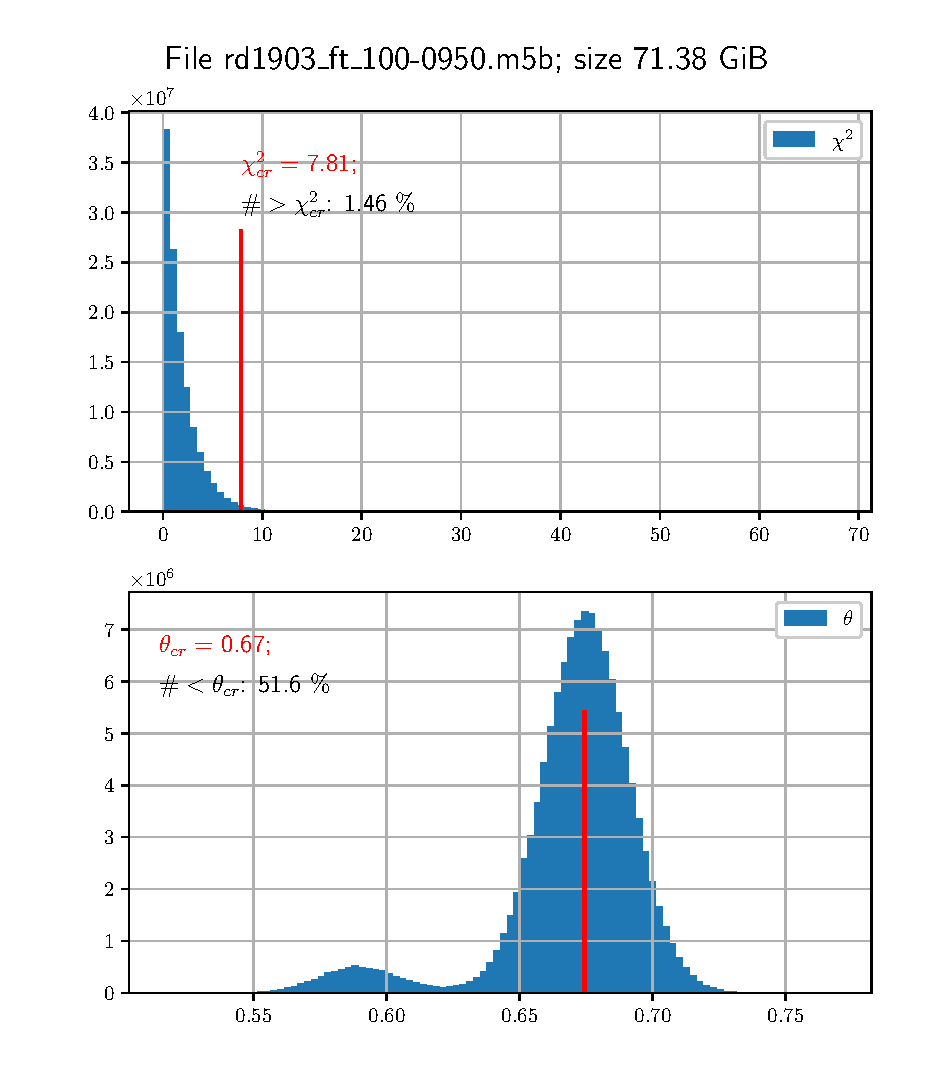
\includegraphics[width=35pc]{fig_chi2_and_thresh_distr_1.eps}
  %\noindent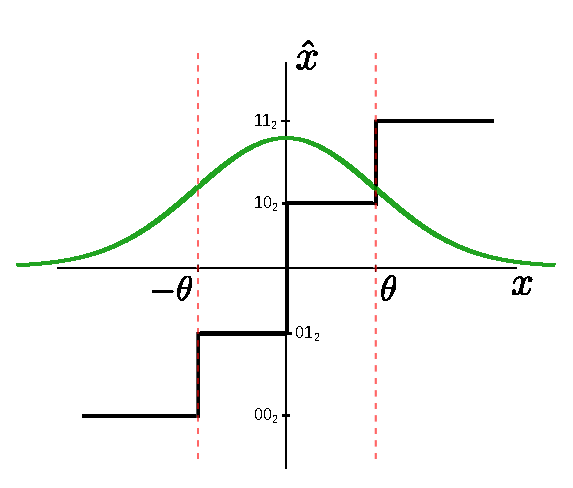
\includegraphics[width=20pc]{fig_4_Level_Quantization_Pattern_impr.eps}
  %\includegraphics[width=\linewidth]{}
  \caption{\small Distributions of $\chi^2$ (upper pane) and $\theta$ (lower pane). The plots are based on the results of normality testing the data from file rd1903\_ft\_100-0950.m5b. The vertical red lines show the positions of $\chi^2_{cr}$ and $\theta_{cr}$. }
  \label{chi2_and_thresh_distr_1}
  \end{center}
\end{figure}


\begin{figure}[ht!]
  \begin{center}
  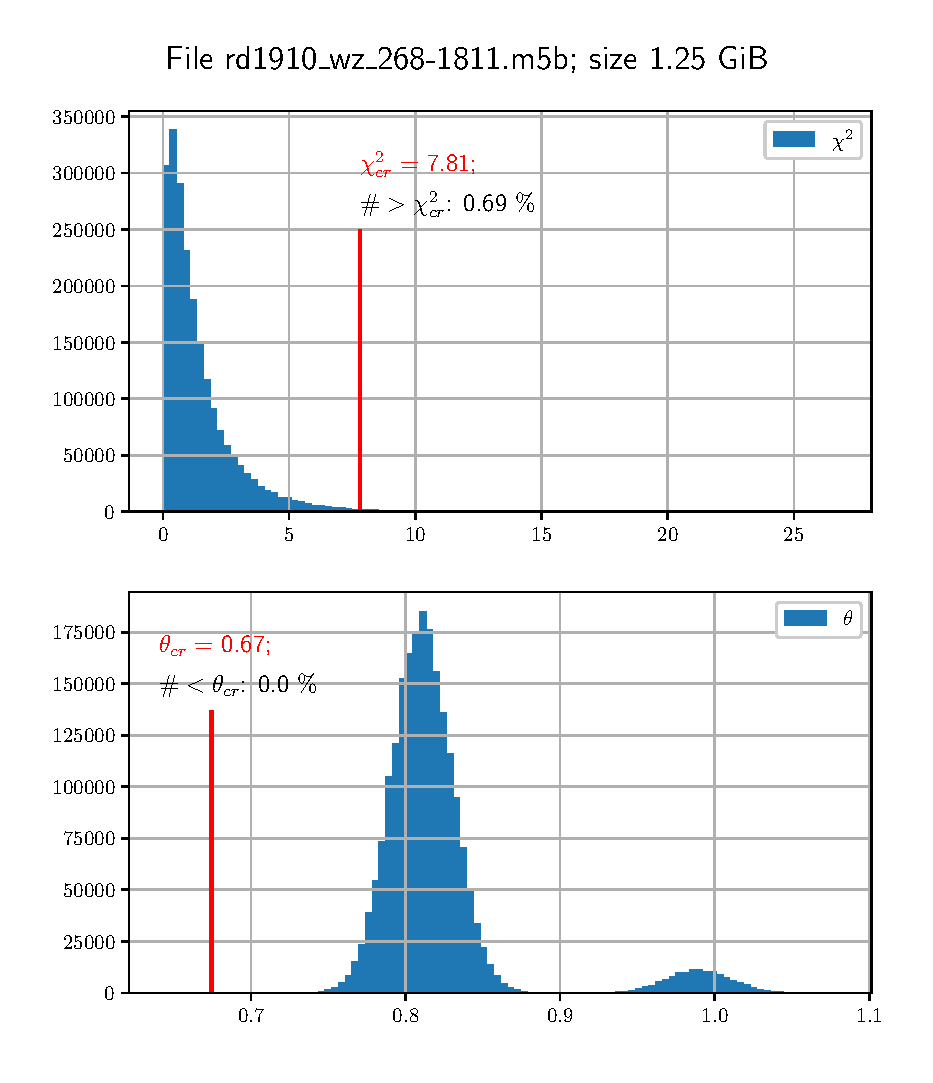
\includegraphics[width=35pc]{fig_chi2_and_thresh_distr_2.eps}
  %\noindent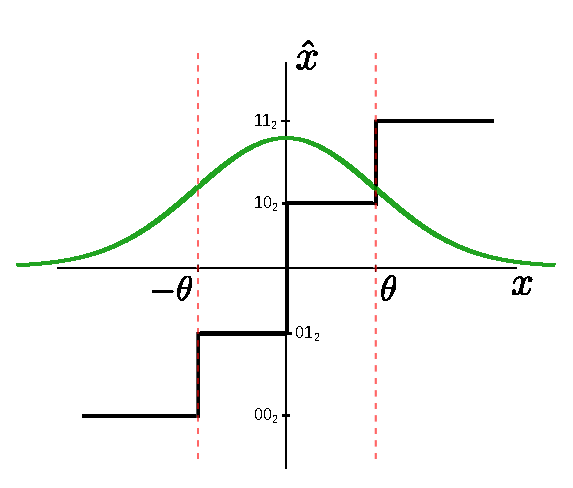
\includegraphics[width=20pc]{fig_4_Level_Quantization_Pattern_impr.eps}
  %\includegraphics[width=\linewidth]{}
  \caption{\small Distributions of $\chi^2$ (upper pane) and $\theta$ (lower pane). The plots are based on the results of normality testing the data from file rd1910\_wz\_268-1811.m5b. The vertical red lines show the positions of $\chi^2_{cr}$ and $\theta_{cr}$. }
  \label{chi2_and_thresh_distr_2}
  \end{center}
\end{figure}


\begin{figure}[ht!]
  \begin{center}
  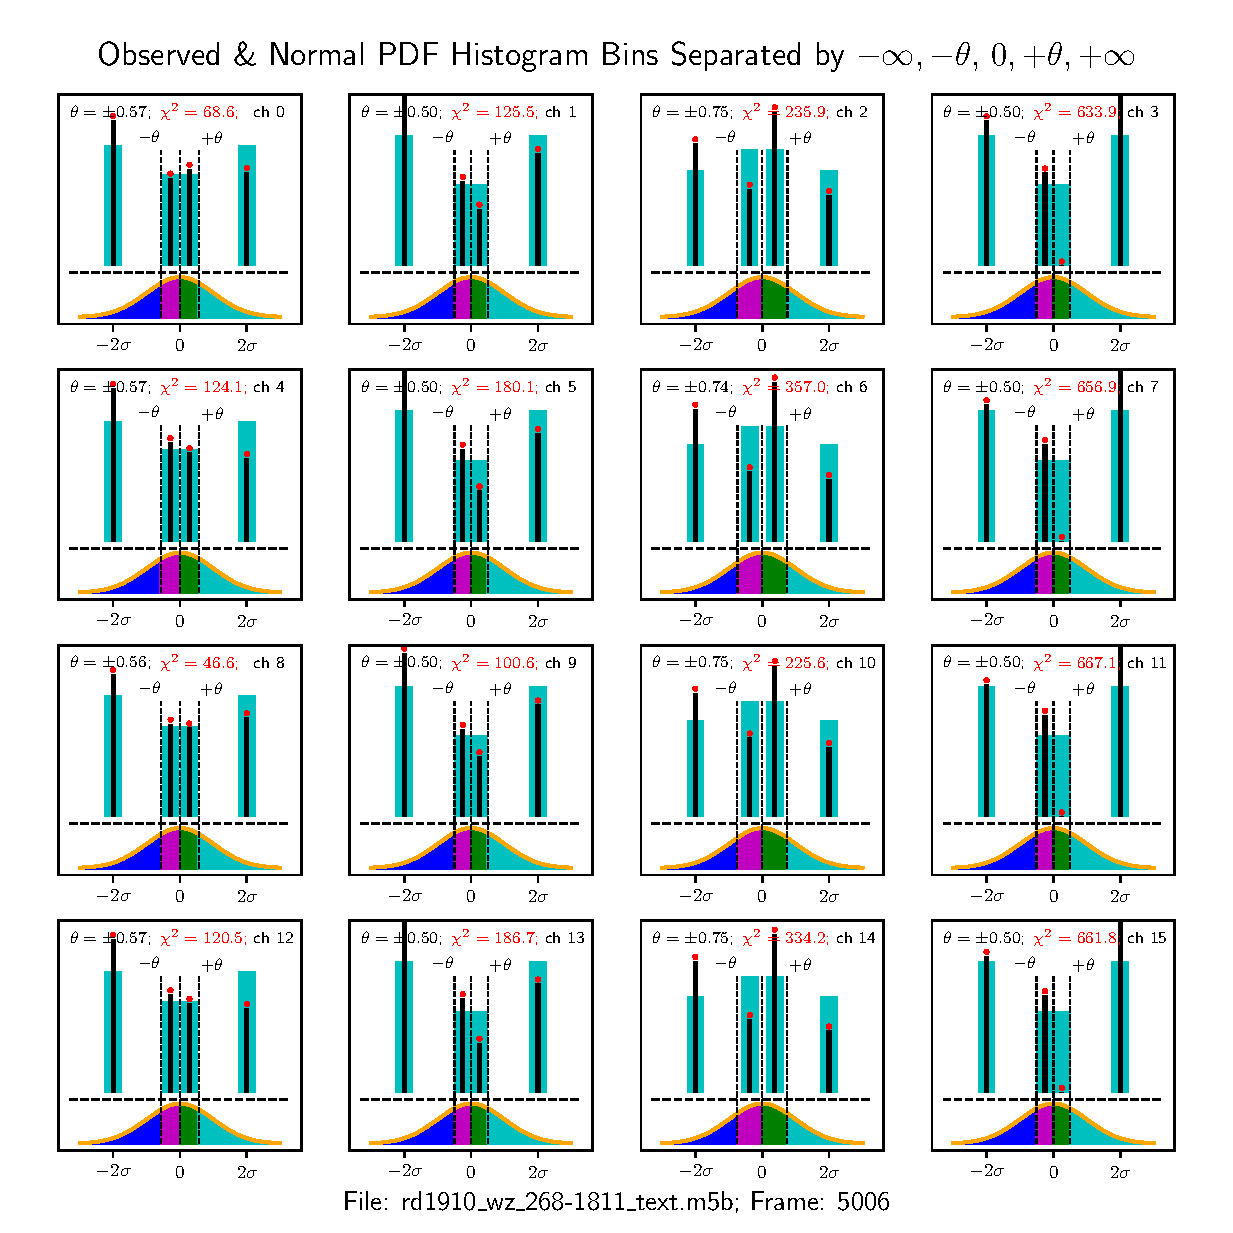
\includegraphics[width=40pc]{fig_4x4_Histograms_text_inserted.eps}
  %\noindent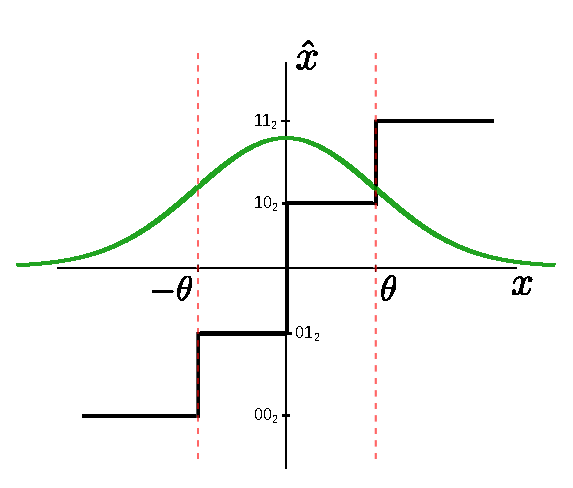
\includegraphics[width=20pc]{fig_4_Level_Quantization_Pattern_impr.eps}
  %\includegraphics[width=\linewidth]{}
  \caption{\small Observed and normal PDF histogram bins separated by $-\infty, -\theta, \, 0, +\theta, +\infty$. The histograms of observed data from an M5B file frame 5006 are shown as narrow black bars with red dots at the tips. The histograms of normal PDF are wider cyan bars. The normal PDFs with colored areas are given below the histograms. Frame 5006 was filled with some UTF-8-coded text, and one can see its distributions are far from the normal.}
  \label{hists_text_4x4}
  \end{center}
\end{figure}



\begin{figure}[ht!]
  \begin{center}
  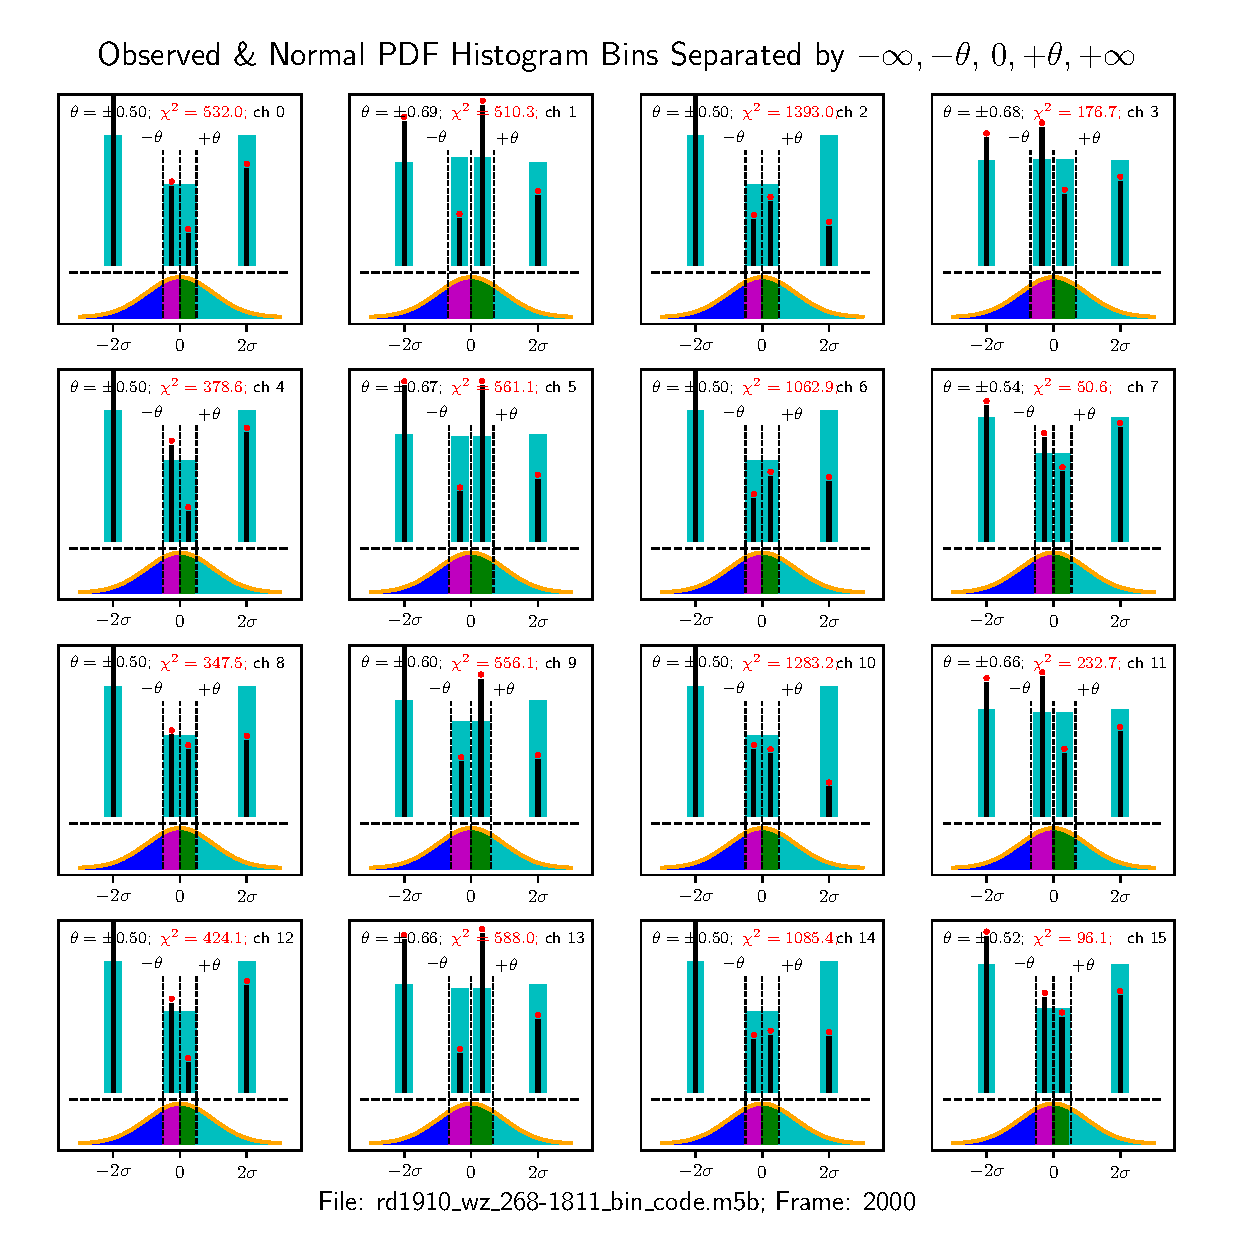
\includegraphics[width=40pc]{fig_4x4_Histograms_bin_code_inserted.eps}
  %\noindent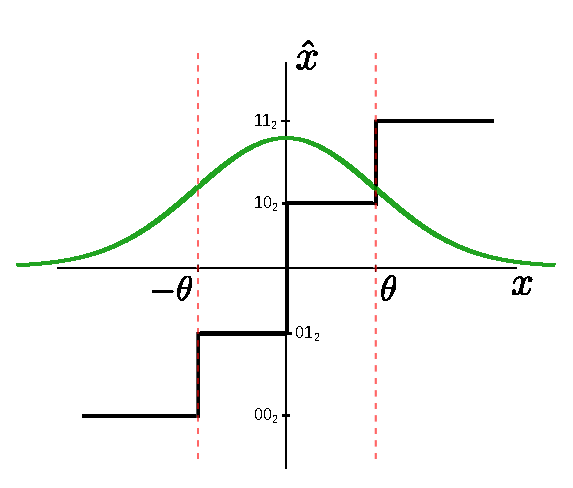
\includegraphics[width=20pc]{fig_4_Level_Quantization_Pattern_impr.eps}
  %\includegraphics[width=\linewidth]{}
  \caption{\small Observed and normal PDF histogram bins separated by $-\infty, -\theta, \, 0, +\theta, +\infty$. The histograms of observed data from an M5B file frame 2000 are shown as narrow black bars with red dots at the tips. The histograms of normal PDF are wider cyan bars. The normal PDFs with colored areas are given below the histograms. Frame 2000 was filled with some binary code (ELF 64-bit LSB executable), and one can see its distributions are far from the normal.}
  \label{hists_bin_code_4x4}
  \end{center}
\end{figure}



\begin{figure}[ht!]
  \begin{center}
  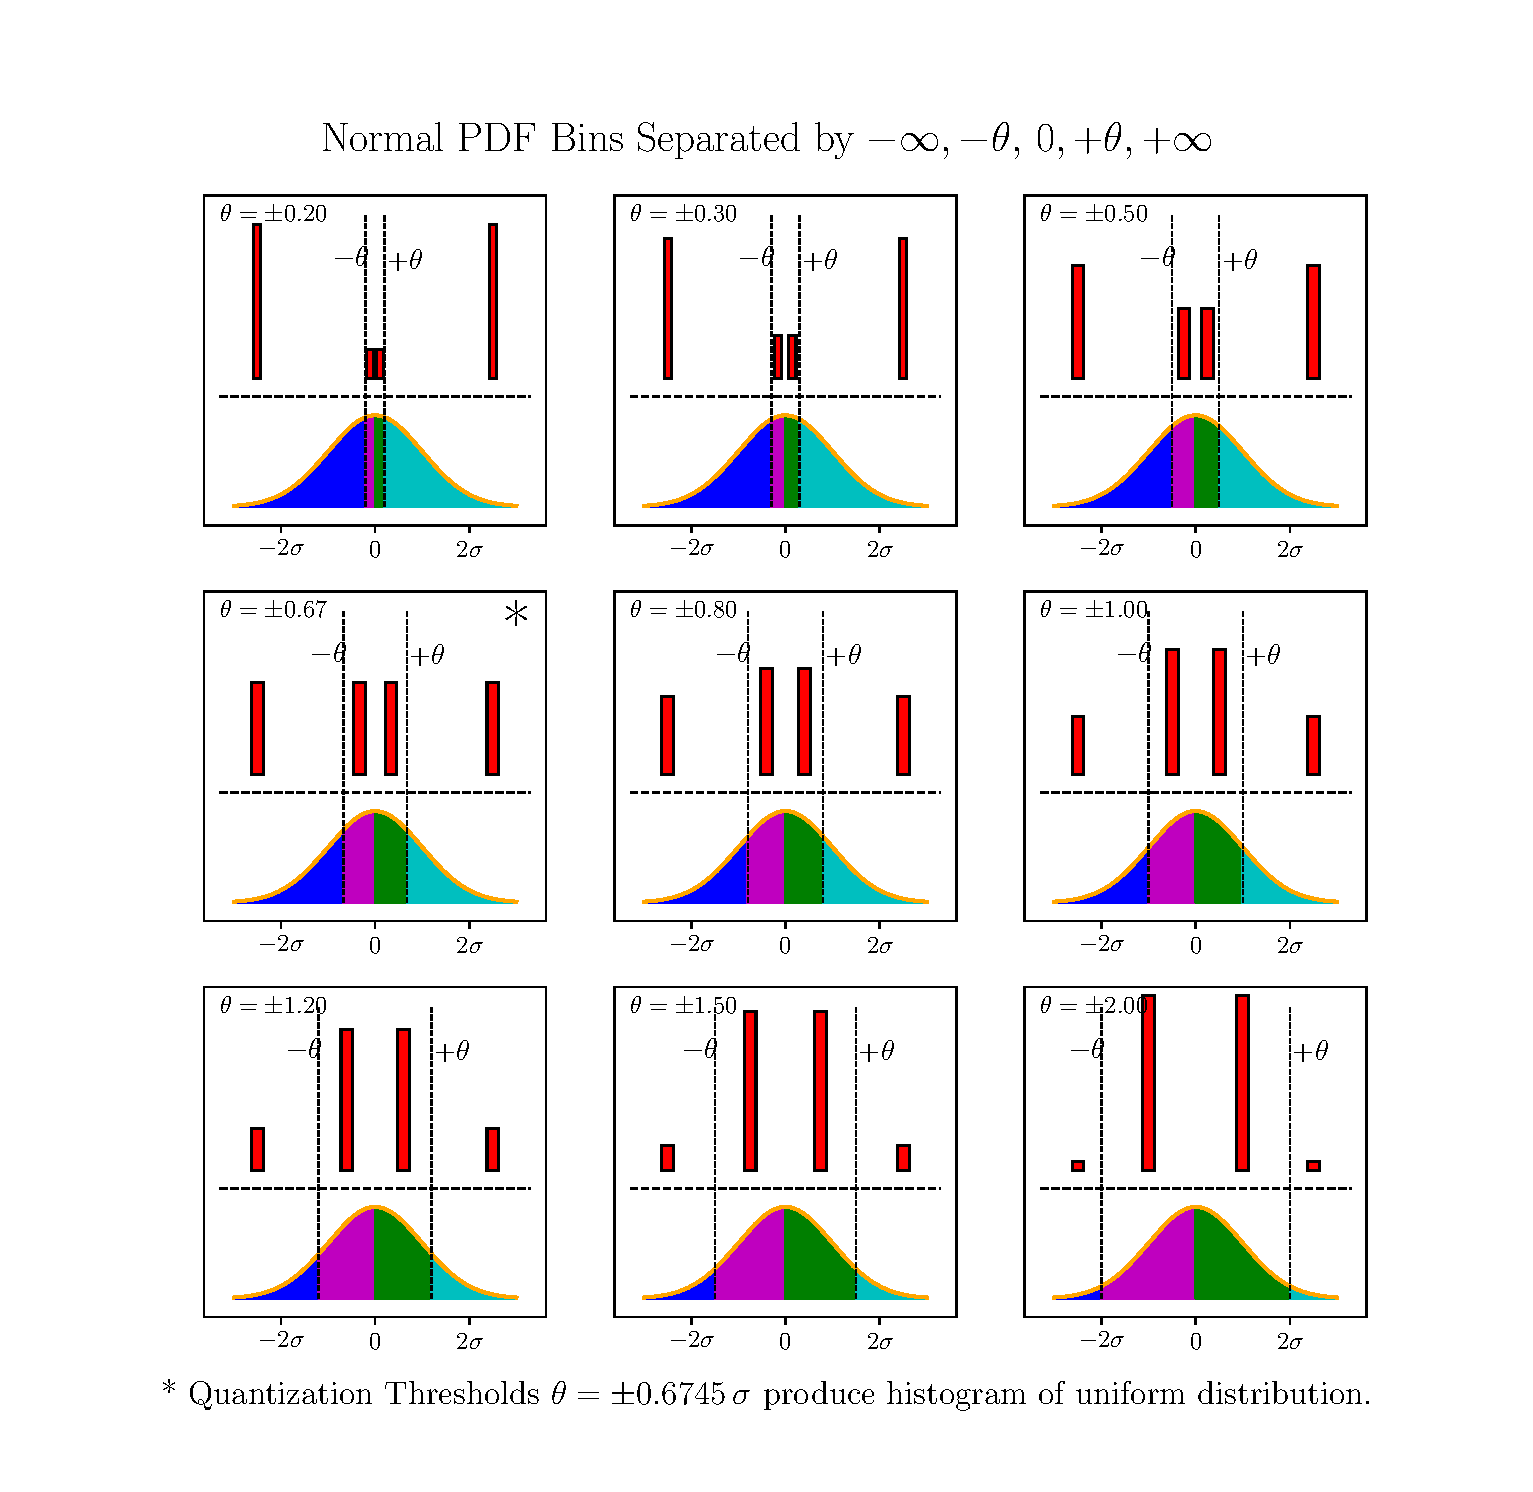
\includegraphics[width=45pc]{fig_various_bin_size_histograms.eps}
  \caption{\small The histograms of standard normal distribution for several different quantization thresholds $\pm\theta = $[0.2, 0.3, 0.5, 0.6745, 0.8, 1.0, 1.2, 1.5, 2.0]. The thresholds $\theta = \pm 0.6745 \, \sigma$ produce histogram of the uniform distribution despite the input analog signal is normal.}
  \label{var_bins_hists}
  \end{center}
\end{figure}



\begin{figure}[ht!]
  \begin{center}
  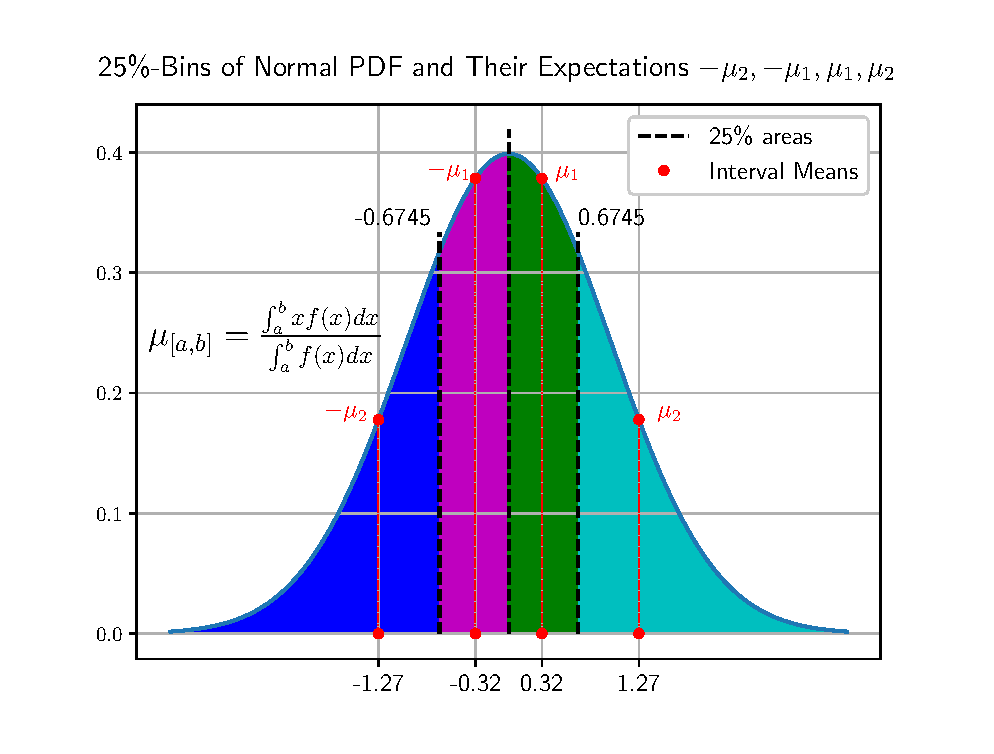
\includegraphics[width=35pc]{fig_25_percent_bins_and_expectations.eps}
  \caption{\small The area under normal PDF curve divided into 4 equal-area bins by the vertical lines at $-\theta_{cr} = -0.6745$, 0, and $\theta_{cr} = +0.6745$. The mathematical expectations of the bins, $\mu_1=\pm 0.32\sigma$ and $\mu_2=\pm 1.27\sigma$ are indicated with red dots.}
  \label{bins_25_pc}
  \end{center}
\end{figure}



\end{document}



